%! TeX program = xelatex

\documentclass[12pt, a4paper]{article}
\usepackage{cmap}
\usepackage[fontsize=12pt]{scrextend}
\usepackage[T2A]{fontenc}
\usepackage[utf8]{inputenc}
\usepackage[english,russian]{babel}
\usepackage{amsmath,amsfonts,amssymb,amsthm,mathtools}
\usepackage[left=20mm, top=20mm, right=20mm, bottom=20mm, nohead, footskip=1cm]{geometry}
\usepackage{multirow}
\usepackage{array}
\usepackage{multicol}
\usepackage{graphicx}
\usepackage{wrapfig}
\usepackage{indentfirst}
\usepackage{enumitem}

\usepackage{polyglossia}
\usepackage{titlesec}
\usepackage{sectsty}
\usepackage{setspace}
\usepackage{fontspec}
\defaultfontfeatures{Mapping=tex-text}

\usepackage{lipsum}
\usepackage{tocloft}
\usepackage[dvipsnames]{xcolor}

\usepackage{caption}
%\captionsetup{labelfont=it, textfont=it}
%\captionsetup[figure]{name=Схема}

\usepackage{hyperref}

\hypersetup{
    colorlinks=false,
    linktoc=all
}
\urlstyle{same}

\setmainlanguage{english}
\setotherlanguage{russian}
\setkeys{russian}{babelshorthands=true}
\setmainfont{Times New Roman}
\newfontfamily\cyrillicfont{Times New Roman}
\let\cyrillicfonttt\ttfamily
%\onehalfspacing

%\allsectionsfont{\centering}
\renewcommand{\cftsecleader}{\cftdotfill{\cftdotsep}}

%======================================SECTIONING=========================================
%\makeatletter
%\renewcommand*\l@section{\@dottedtocline{1}{1.5em}{2.3em}}
%\makeatother
%======================================SECTIONING=========================================

\pretolerance=6000
\tolerance=3000
\emergencystretch=4pt

\setlength\intextsep{10pt}

\graphicspath{{./visuals/}}
\setlength{\parskip}{0.3125cm}
\setlength{\parindent}{1.25cm}
\setlength{\columnsep}{1cm}
\author{Grigoryev Mikhail}
\title{Algs lab}

\begin{document}

\thispagestyle{empty}

\vspace{30mm}

\begin{center}
FEDERAL STATE AUTONOMOUS EDUCATIONAL INSTITUTION \\
OF HIGHER EDUCATION \\
ITMO UNIVERSITY

\vspace{40mm}

{\large \textbf{Report \\
on the practical task No. 2 \\
"Algorithms for unconstrained nonlinear optimization. Direct methods"}}
\end{center}

\vspace{15mm}

\begin{flushright}
{\large Performed by \\
\textit{Mikhail Grigoryev \\
Academic group J4133c \\}
Accepted by \\
Dr Petr Chunaev}
\end{flushright}

\vspace{100mm}

\begin{center}
St. Petersburg \\
2022
\end{center}

\newpage

\section*{Goal}
\addcontentsline{toc}{section}{Goal}

The use of direct methods (one-dimensional methods of exhaustive search, dichotomy, golden section search; multidimensional methods of exhaustive search, Gauss (coordinate descent), Nelder-Mead) in the tasks of unconstrained nonlinear optimization.

\section*{Formulation of the problem}
\addcontentsline{toc}{section}{Formulation of the problem}

\textbf{Task 1.} Using one-dimensional methods of exhaustive search, dichotomy and golden section search an approximate solution (with precision $\varepsilon = 0.001$) for the minima $x: \quad f(x) \to min$ of the following functions and domains should be found:
\begin{enumerate}
	\item $f(x) = x^3, \quad x\in [0, 1]$;
	\item $f(x) = |x-0.2|, \quad x\in [0, 1]$;
	\item $f(x) = x\sin \frac{1}{x}, \quad x\in [0.01, 1]$.
\end{enumerate}
Calculate the number of $f$-calculations and the number of iterations performed in each method and analyze the results. Explain differences (if any) in the results obtained.

\textbf{Task 2.} Generate random numbers $\alpha \in (0, 1)$ and $\beta \in (0, 1)$. Furthermore, generate the noisy data $\{ x_k, y_k \}$, where $k = 0, \cdots, 100$, according to the rule:
\[ y_k = \alpha x_k + \beta + \delta_k, \quad x_k = 0.01 k, \]
where $\delta_k ~ N(0, 1)$ are values of a random variable with standard normal distribution. Approximate the data by the following linear and rational functions:
\begin{enumerate}
	\item $F(x, a, b) = ax + b$,
	\item $F(x, a, b) = \frac{a}{1+bx}$,
\end{enumerate}
by means of least squares through the numerical minimization (with precision $\varepsilon = 0.001$) of the following function:
\[ D(a, b) = \sum_{k=0}^{100} \left( F(x_k, a, b) - y_k \right)^2 \]
To solve the minimization problem, use the methods of exhaustive search, Gauss and Nelder-Mead. If necessary, set the initial approximations and other parameters of the methods. Visualize the data and the approximants obtained in a plot separately for each for each type of \textbf{approximant} so that one can compare the results for the numerical methods used. Analyze the results obtained (in terms of number of iterations, precision, number of iterations, etc.).

\newpage

\section*{Brief theoretical part}
\addcontentsline{toc}{section}{Brief theoretical part}

Optimization methods are essentially methods of finding optimal (depens on the task) values of target functions. Often optimization is just minimizing a certain function.

The solution to the optimization (minimization) problem is finding:
\[ x^* \in Q: \quad f(x^*) = \min_{x\in Q} f(x) \def \arg \min_{x\in Q} f(x) \]
Finding the argument which corresponds to the function minimum will let us find the value of the function at its minimum.

In this practical work local minima will be found, $f(x)$ can be nonlinear and no additional constrictions on the argument will be applied. Hence the title, "unconstrained nonlinear optimization".

In addition to that, in this work only direct methods will be used, in other words, only values of $f(x)$ (and no derivatives) will be used. Those methods can be utilized on continuous functions, which are not necessarily differentiable.

In the first task, all three method of one-dimensional optimization were implemented by scratch: 
\begin{enumerate}
	\item exhaustive search simply by means of nested loops and local variables \textit{current\_min\_x} and \textit{current\_min\_y}, where current minimal parameters were kept;
	\item dichotomic search was implemented recursively, each time with a smaller domain (computation stops when domain is smaller than $\varepsilon$);
	\item golden section search was implemented similarly (recursion with a constantly narrowing domain), one of the pivot points was kept as a function parameter so as to save computations.
\end{enumerate}

In the second task:
\begin{enumerate}
	\item exhaustive search was implemented via nested loops, deviation function was computed for every single point in $\alpha \beta$ space, point with smaller deviation than former ones were saved to local variables;
	\item Gauss search was implemented in such a way that one-dimensional optimizations were solved by dichotomic search from task 1;
	\item Nelder-Mead search was taken from SciPy library.
\end{enumerate}

\newpage

\section*{Results}
\addcontentsline{toc}{section}{Results}

\textbf{Task 1.} One-dimensional methods of exhaustive search, dichotomy and golden-section were used to find minima of:
\[ f(x) = x^3 \qquad f(x) = |x-0.2| \qquad f(x) = x\sin \frac{1}{x} \]
within domains
\[ x\in [0,1] \qquad x\in [0,1] \qquad x\in [0.01, 1] \]
respectively.

In cases of all three functions all three methods converged to the same minima:
\begin{center}
\begin{tabular}{cccc}
\hline
alg/func   & $x^3$            & $|x-0.2|$        & $x\sin (1/x)$     \\ \hline
Exhaustive & (0.0000, 0.0000) & (0.2000, 0.0000) & (0.2230, -0.2172) \\
Dichotomic & (0.0000, 0.0000) & (0.1996, 0.0004) & (0.2221, -0.2172) \\
Golden     & (0.0000, 0.0000) & (0.1997, 0.0003) & (0.2223, -0.2172) \\ \hline
\end{tabular}
\end{center}
As for numbers of iterations, exhaustive search took 1000 iterations and thus 1000 function calls (except it took 900 iterations and calls for the last function due to the narrower domain). Dichotomic search always took 12 iterations and 24 calls. Golden-section search always took 16 iterations and 32 calls.

Judging solely by iteration number/call number, exhaustive search seems useless, as it takes much more iterations to find the minimum. Dichotomic search almost halves the domain every iteration, thus is much more efficient. Golden-section search is close to dichotomic in terms of numbers of iterations and function calls. Golden-section search also requires less domain pivot points to be calculated, which could be beneficial on large domains.

\textbf{Task 2.} Random parameters for generating noisy data were generated. They are shown below:
\[ \alpha = 0.9290 \qquad \beta = 0.5443 \]
Three methods of linear approximation were applied to the problem, the data obtained is presented in the table:
\begin{center}
\begin{tabular}{cccc}
\hline
alg/param   & (A, B)           & Iterations & Function calls \\ \hline
Exhaustive  & (0.3283, 0.8759) & 1000000    & 1000000        \\
Gauss       & (0.3309, 0.8741) & 875        & 2520           \\
Melder-Mead & (0.3285, 0.8756) & 32         & 60             \\ \hline
\end{tabular}
\end{center}
All three methods gave close results, as expected (no non-linearity). Exhaustive search took a million iterations and function calls to compute, as Gauss took under a thousand iterations and about three times that function calls. Melder-Mead converged in mere 32 iterations and 60 calls. Thus, Melder-Mead deemed itself very useful for linear approximation.

\newpage

\begin{figure}[!h]
\centering
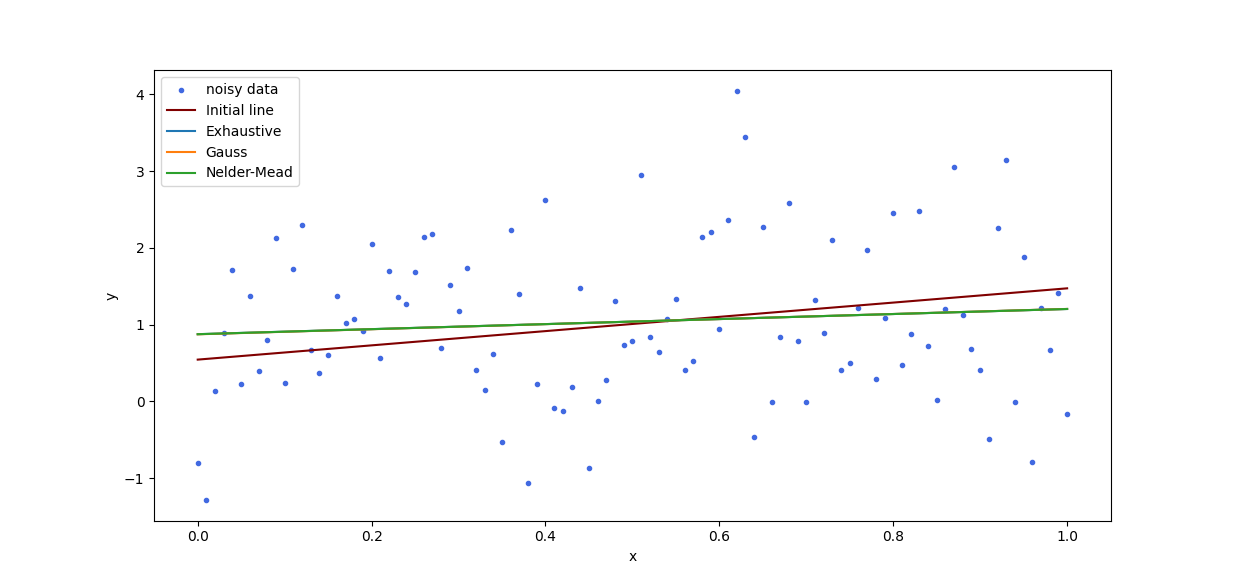
\includegraphics[width=\textwidth]{line1.png}
\caption{Results of applying exhaustive, Gauss and Nelder-Mead searches to solve the problem of linear approximation.}
\end{figure}

\begin{figure}[!h]
\centering
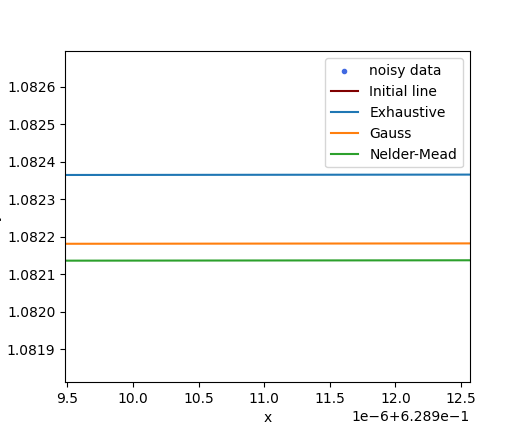
\includegraphics[width=0.45\textwidth]{line2.png}
\caption{Close linear approximations zoomed.}
\end{figure}

Random parameters for rational approximation were:
\[ \alpha = 0.1316 \qquad \beta = 0.0080 \]
Obtained data is presented below:
\begin{center}
\begin{tabular}{cccc}
\hline
alg/param   & (A, B)            & Iterations & Function calls \\ \hline
Exhaustive  & (0.1271, 1.0000)  & 1000000    & 1000000        \\
Gauss       & (0.1264, 1.0000)  & 75         & 216            \\
Melder-Mead & (0.9232, 22.3244) & 62         & 117             \\ \hline
\end{tabular}
\end{center}
Obviously, Melder-Mead converged to a completely different curve than exhaustive and Gauss methods. Those two showed similar results with vastly different iteration and call numbers. Exhaustive search took 1000000 iterations and calls, when Gauss converged in 75 iterations and 216 calls. Thus, Gauss seemed much more useful than exhaustive search method. It's complicated to compare Melder-Mead to the former methods due to its unpredictable results on non-linear approximation. However, it converged faster: 62 iterations and 117 calls.

\begin{figure}[!h]
\centering
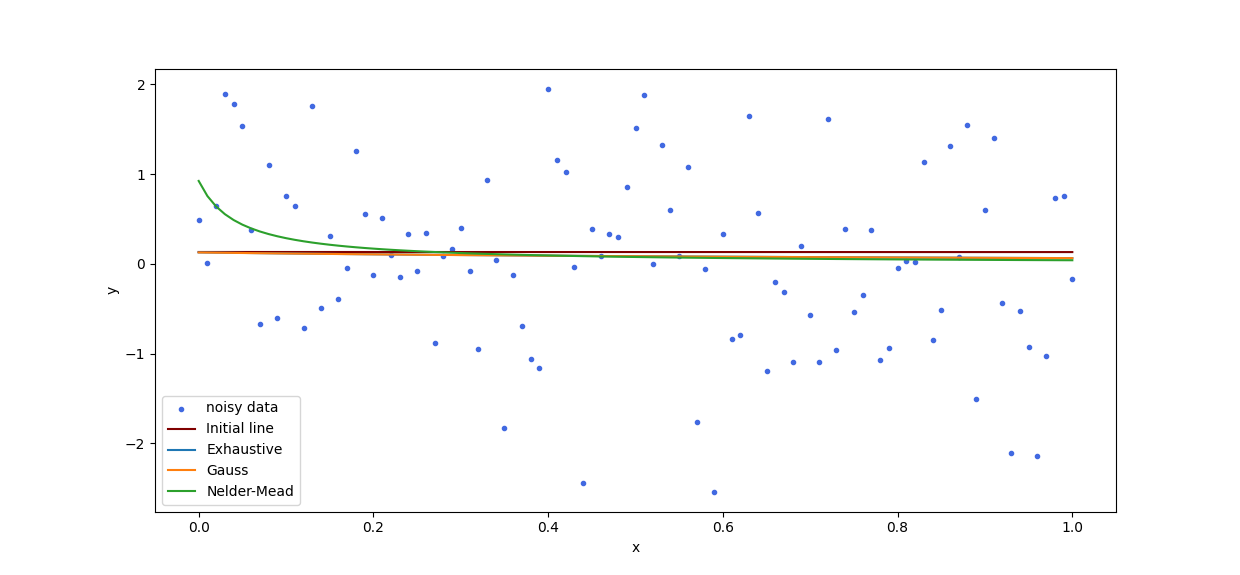
\includegraphics[width=\textwidth]{rational1.png}
\caption{Results of applying exhaustive, Gauss and Nelder-Mead searches to solve the problem of rational approximation.}
\end{figure}

\begin{figure}[!h]
\centering
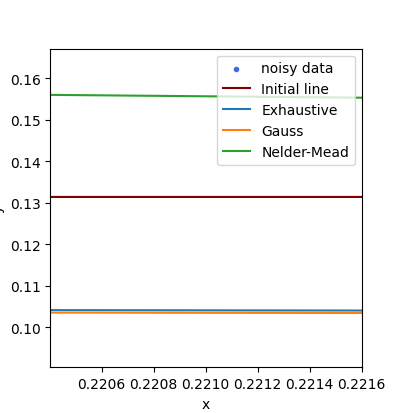
\includegraphics[width=0.45\textwidth]{rational2.png}
\caption{Close rational approximations zoomed.}
\end{figure}

\section*{Conclusions}
\addcontentsline{toc}{section}{Conclusions}

One-dimensional (exhaustive, dichotomic and golden-section searches) and multidimensional (exhaustive, Gauss and Nelder-Mead searches) methods were implemented and applied to tasks of unconstrained nonlinear optimization, tested against each other and compared in terms of perfomance.

\newpage

\section*{Appendix}
\addcontentsline{toc}{section}{Appendix}

GitHub link for task 1: \url{https://github.com/Dormant512/itmo_lab_listings/blob/main/lab2_task1.py}.

GitHub link for task 2: \url{https://github.com/Dormant512/itmo_lab_listings/blob/main/lab2_task2.py}.

\begin{figure}[!h]
\centering

\includegraphics[width=0.3\textwidth]{lab2task1.png}

\includegraphics[width=0.3\textwidth]{lab2task2.png}
\end{figure}


\end{document}
